% this file is called up by thesis.tex
% content in this file will be fed into the main document

%: ----------------------- name of chapter  -------------------------
\chapter{Planning 3D Motions for Torpedo-shaped and Propeller-driven AUVs}
\label{ch:planning_3D} %
% top level followed by section, subsection


%: ----------------------- paths to graphics ------------------------

% change according to folder and file names
\ifpdf
    \graphicspath{{4_planning_3D/figures/PNG/}{4_planning_3D/figures/PDF/}{4_planning_3D/figures/}}
\else
    \graphicspath{{4_planning_3D/figures/EPS/}{4_planning_3D/figures/}}
\fi

%: ----------------------- contents from here ------------------------

Although there is an important number of \ac{AUV} applications in which the
vehicle navigates at a constant altitude or depth, and therefore a \ac{2D}
path/motion planning approach is valid, there are other scenarios in which the
vehicle is required to conduct \ac{3D} motions (see
Chapters~\ref{ch:introduction}~and~\ref{ch:state_of_the_art}).
Chapter~\ref{ch:motion_constratins} presented two alternative approaches to plan
collision-free paths, which take into account the motion constraints of a
torpedo-shaped \ac{AUV}. While both approaches are limited to plan \ac{2D}
paths, the one that uses Dubins curves also allows to obtain near-optimal
solutions.

In order to define a correct strategy for planning \ac{3D} \ac{AUV} paths, it is
necessary to firstly establish the specific vehicle type, and then to understand
its main motion characteristics. Underwater gliders, for instance, always
require \ac{3D} motion planners and controllers, especially if considered their
propulsion mechanism and the kind of trajectories they follow (see
Chapter~\ref{ch:introduction}, Fig.~\ref{fig:GliderAUV}). However, given that
they operate in open sea areas, these vehicles do not usually have to deal with
obstacles, narrow passages, or high-relief environments. Instead, their motion
planners are more focused on coping with external perturbations such as ocean
currents, which may deviate the glider from the desired trajectory. This makes
that, in most cases, motion planning becomes a trajectory planning problem,
which must consider the ocean forecast in order to minimize the effect of such
perturbations~\cite{Smith2010,Thompson2010}.

Propeller-driven \acp{AUV}, on the other hand, are equipped with thrusters that
increase their maneuverability for \ac{2D} and \ac{3D} motions. This chapter
discusses the \ac{3D} first-order model, which approximately describes the
kinematic behavior of a torpedo-shaped and propeller-driven \ac{AUV}. It also
analyses the motion constraints involved, and how they can be included into a
extended version of the Dubins curves approach presented in the previous
chapter.

\section{3D First-Order Motion Model}

For \ac{3D} motions, six different variables specify the vehicle's position
and orientation, which means that the \ac{C-Space} is $\mathcal{C} = SE(3) =
\mathbb{R}^3 \times SO(3)$ (see Fig.~\ref{fig:RefFramesAUV3D}). Dynamic models,
which normally consider all the $6$ variables, have also been used in some
\ac{AUV} path-planning applications~\cite{Ying2000,Wehbe2014}. Nonetheless, and
as it has been already mentioned, their high computational cost make them an
inappropriate alternative for the scenarios proposed in this thesis.

As occurs with \ac{2D} \ac{AUV} motions, there exist different kinematic models
that could be used for describing \ac{3D} motions. They mainly vary according to
the \ac{AUV} motion mechanism and its corresponding constraints. Two different
cases will be explained in the following sections, one of which has been
employed for planning collision-free paths for the Sparus~II \ac{AUV}.

\begin{figure}[htbp]
	\centering
	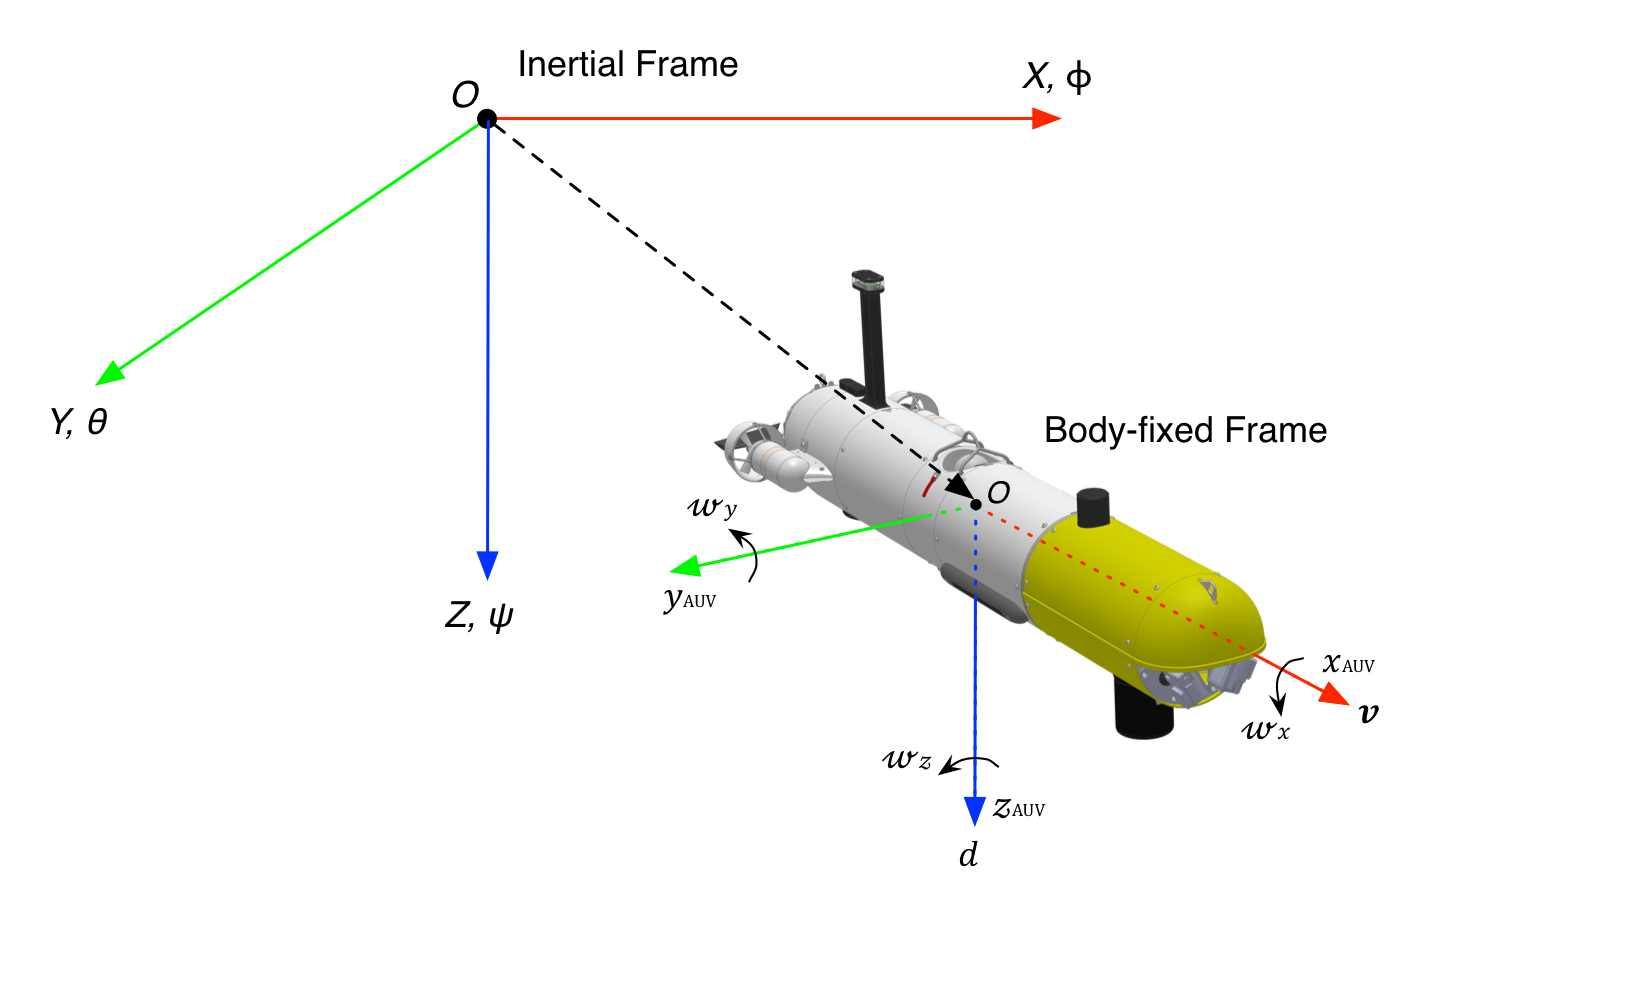
\includegraphics[width=.9\linewidth]{RefFramesAUV3D} \quad
\caption[Perspective view of the Sparus~II AUV, including the inertial and
body-fixed frames, and the 6D vehicle state and control variables.]
{Perspective view of the Sparus~II AUV, including the inertial and
body-fixed frames, and the 6D vehicle state and control variables.}
\label{fig:RefFramesAUV3D}
\end{figure}

\subsection{Vertical Motion Constraints}

As explained in Section~\ref{sec:2d_kinematic_model}, a torpedo-shaped and
propeller-driven \ac{AUV} that conducts \ac{2D} motions, is generally subject to
differential (motion) constraints. These constraints prevent the vehicle from
laterally moving by only allowing it to turn while moving forward or backward,
or to spin over when it is equipped with two back thrusters, for example as
occurs with the Sparus~II. When analysing \ac{3D} motions for this kind of
vehicles, such limitations must be combined with those imposed by the mechanism
that permits the vehicle ascending and descending.

Since the \ac{AUV} volume remains constant during a mission, it is necessary to
increase the downward force in order to make the vehicle vary its
navigation depth. For doing so, there are different submerging mechanisms that
can be classified into two groups. \begin{inparaenum}[1)]
\item Those vehicles with only one propulsion force in the back, which
must be distributed into forward and downward components. This can be done
either with inner ballast systems or with external foreplanes.
\item Those vehicles with two propulsion forces, one for forward motion, and an
independent one for submerging, which is commonly generated by one or more
vertical thrusters.
\end{inparaenum}

From the kinematics perspective, both groups generate different kind of motion
constraints. The former group's vehicles descend and ascend with a non-zero
pitch angle. In this case, the maximum surge speed and the pitch angles
establish the maximum descending and ascending speeds. The second group's, on
the other hand, are normally designed and trimmed for diving with a near-zero
pitch angle. In this case, the maximum descending and ascending speeds are
determined by the vertical thruster(s) specifications. In both cases, the
vehicles are normally equipped with additional aft planes to generate turning
maneuvers, and to minimize the vehicle roll. These two approaches result into
different mathematical equations that describe the vehicle kinematics.

% \begin{figure}[htbp]
% \myfloatalign
%     \subfloat[Descending With Pitch.]
%     {\label{fig:DescendingWithPitch}%
%      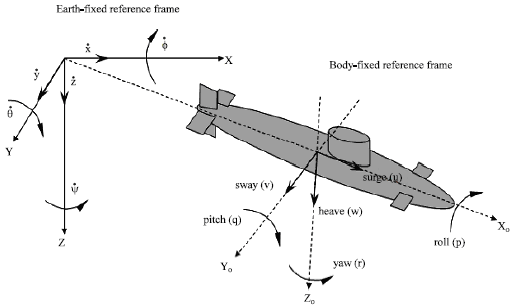
\includegraphics[width=.45\linewidth]{DescendingWithPitch}} \quad
%     \subfloat[Descending Without Pitch]
%     {\label{fig:DescendingWithoutPitch}
%     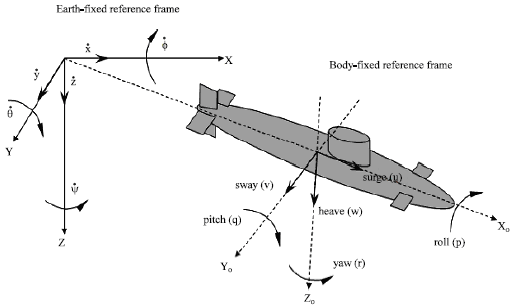
\includegraphics[width=.45\linewidth]{DescendingWithPitch}}
% \caption{\hl{Descending}.}
% \label{fig:DescendingPitch}
% \end{figure}

\subsection{Mathematical Formulation}

A torpedo-shaped \ac{AUV} with non-zero pitch vertical motion, can be
kinematically described with a 6-\ac{DOF} model as follows~\cite{Wadoo2010}:

\begin{equation}
\label{eq:Full6DOFKinEqAUV3D}
\begin{split}
	\begin{bmatrix}
		\dot{x}\\
		\dot{y}\\
		\dot{z}\\
		\dot{\phi}\\ 
		\dot{\theta}\\
		\dot{\psi}\\
	\end{bmatrix} & =
	\begin{bmatrix}
		cos\left(\psi\right)cos\left(\theta\right) & 0 & 0 & 0\\
		sin\left(\psi\right)cos\left(\theta\right) & 0 & 0 & 0\\
		-sin\left(\theta\right) & 0 & 0 & 0\\
		0 & 1 & sin\left(\phi\right)tan\left(\theta\right) & cos\left(\phi\right)tan\left(\theta\right)\\
		0 & 0 & cos\left(\phi\right) & -sin\left(\phi\right)\\
		0 & 0 & sin\left(\phi\right)sec\left(\theta\right) & cos\left(\phi\right)sec\left(\theta\right)\\
	\end{bmatrix}
	\begin{bmatrix}
		v\\
		w_x\\
		w_y\\
		w_z\\
	\end{bmatrix}\\
	& = \begin{bmatrix}
		v\ cos\left(\psi\right)cos\left(\theta\right)\\
		v\ sin\left(\psi\right)cos\left(\theta\right)\\
		-v\ sin\left(\theta\right)\\
		w_x + w_y\ sin\left(\phi\right)tan\left(\theta\right) +
		w_z\ cos\left(\phi\right)tan\left(\theta\right)\\
		w_y\ cos\left(\phi\right) -w_z\ sin\left(\phi\right)\\
		w_y\ sin\left(\phi\right)sec\left(\theta\right) + w_z\ cos\left(\phi\right)sec\left(\theta\right)\\
	\end{bmatrix}
	\text{,}
\end{split}
\end{equation}

where $q=\left[x, y, z, \phi, \theta, \psi\right]^T$ corresponds to the system
state that includes its \ac{3D} position and orientation with respect to an
inertial reference frame, and $\dot{q}=\left[\dot{x}, \dot{y}, \dot{z}, \dot{\phi},
\dot{\theta}, \dot{\psi}\right]^T$ is the first time derivative that depends on
the state itself and the control inputs, \ie linear/surge speed ($v$) and
turning rates around the different vehicle axis ($w_x, w_y, w_z$). Here the
vehicle is subject to two non-holonomic constraints, which are established
on the linear velocities along the vehicle $y$ and $z$ directions.This full
kinematic model presented in Eq.~\eqref{eq:Full6DOFKinEqAUV3D}, has been used in
trajectory planning applications~\cite{Qu2009}. However, it can also be
simplified if the vehicle is assumed to maintain a near-zero roll angle ($\phi
\approx 0$):

\begin{equation}
\label{eq:Full5DOFKinEqAUV3D}
\begin{split}
	\begin{bmatrix}
		\dot{x}\\
		\dot{y}\\
		\dot{z}\\
		\dot{\theta}\\
		\dot{\psi}\\
	\end{bmatrix} & = \begin{bmatrix}
		v\ cos\left(\psi\right)cos\left(\theta\right)\\
		v\ sin\left(\psi\right)cos\left(\theta\right)\\
		-v\ sin\left(\theta\right)\\
		w_y\\
		w_z\ cos\left(\phi\right)sec\left(\theta\right)\\
	\end{bmatrix}
\end{split}
\end{equation}

On the other hand, torpedo-shaped and propeller-driven \acp{AUV} with near-zero
pitch motion ($\theta \approx 0$), \ie those with an independent propulsion
force for vertical motion, must be described with a different kinematic model as
follows:

\begin{equation}
\label{eq:Full5DOFKinVertMot}
\begin{split}
	\begin{bmatrix}
		\dot{x}\\
		\dot{y}\\
		\dot{z}\\
		\dot{\phi}\\ 
		\dot{\psi}\\
	\end{bmatrix} & =
	\begin{bmatrix}
		cos\left(\psi\right) & 0 & 0 & 0 & 0\\
		sin\left(\psi\right) & 0 & 0 & 0 & 0\\
		0 & 1 & 0 & 0 & 0\\
		0 & 0 & 1 & 0 & 0\\
		0 & 0 & 0 & sin\left(\phi\right) & cos\left(\phi\right)\\
	\end{bmatrix}
	\begin{bmatrix}
		v\\
		d\\
		w_x\\
		w_y\\
		w_z\\
	\end{bmatrix}\\
	& = \begin{bmatrix}
		v\ cos\left(\psi\right)\\
		v\ sin\left(\psi\right)\\
		d\\
		w_x\\
		w_y\ sin\left(\phi\right) + w_z\ cos\left(\phi\right)\\
	\end{bmatrix}
	\text{,}
\end{split}
\end{equation}

where, once again, $q=\left[x, y, z, \phi, \psi\right]^T$ corresponds to the
system state that includes its position and orientation with respect to an
inertial reference frame. Furthermore, $\dot{q}=\left[\dot{x}, \dot{y}, \dot{z},
\dot{\phi}, \dot{\psi}\right]^T$ is the first time derivative that depends on
the state itself and the control inputs, which in this case are the linear
speeds (surge and  heave $(v, d)$) and the turning rates ($w_x, w_z$). Here the
vehicle is subject to one non-holonomic constraint, which is established on the
linear velocity along the vehicle $y$ direction.
Equation~\eqref{eq:Full5DOFKinVertMot} can also be simplified if the vehicle is
assumed to maintain a near-zero roll angle ($\phi \approx 0$):

\begin{equation}
\label{eq:Full4DOFKinVertMot}
\begin{split}
	\begin{bmatrix}
		\dot{x}\\
		\dot{y}\\
		\dot{z}\\ 
		\dot{\psi}\\
	\end{bmatrix} & =
	\begin{bmatrix}
		v\ cos\left(\psi\right)\\
		v\ sin\left(\psi\right)\\
		d\\
		w\\
	\end{bmatrix}
	\text{,}
\end{split}
\end{equation}

which can be written in the form $\dot{q}=f\left(q,u\right)$, where $q=\left[x,
y, z, \psi\right]^T$, $\dot{q}=\left[\dot{x}, \dot{y}, \dot{z},
\dot{\psi}\right]^T$, and the control input $u=\left[v, d, w\right]^T$ that
corresponds to the surge speed ($v$), the heave speed ($d$), and the rate of
turn ($w$).

\section{Tree Expansion using Dubins Curves for 3D Motions}

Different authors have used Eq.~\eqref{eq:Full4DOFKinVertMot} to generate
\ac{3D} motions for torpedo-shaped and propeller-driven \acp{AUV}. For instance,
Heo \etal presented an approach to build a tree of collision-free and feasible
configurations, over which a final path is found with the A*
algorithm~\cite{Heo2013}. The tree expansion is done by directly integrating
Eq.~\eqref{eq:Full4DOFKinVertMot}, similarly as it was explained in
Sec.~\ref{sec:expan_2d_diff_eq}. However, although A* finds the best solution
over the available paths, it requires an estimate of the cost to the goal, and
this may be hard to obtain, especially in partially known environments.

An alternative to find better \ac{3D} solution paths is to use the \ac{RRT*}
algorithm, however it requires a steering function for improving the
configurations connections (see Sec.~\ref{sec:SamplOptimalPlan}).
Section~\ref{sec:expan_2d_dubins} introduced the use of the Dubins curves as a
steering function for \ac{2D} paths, which can also be extended to
\ac{3D} motions. To do so, let us consider the \ac{AUV} has an independent
propulsion force for its vertical motion, and therefore its kinematics can be
described with Eq.~\eqref{eq:Full4DOFKinVertMot}. In this case, it is possible
to affirm that the motion in the horizontal plane can be decoupled from the
heave (vertical) motion. This allows to directly deal with the former component
as stated in Chapter~\ref{ch:motion_constratins}, while treating the latter
component as an additional constraint over an extended \ac{C-Space},
$\mathcal{C} = SE(2) \times \mathbb{R}$. This motion separation is not new for
underwater vehicles, since it has also been done for dynamic models
formulations~\cite{Miskovic2010}.

On this basis, the path between two states for the \ac{3D} decoupled kinematics
of our vehicle is the one that connects their components in the horizontal plane
using Dubins curves, and their vertical components with a linear interpolation.
The vertical motion must have a gradient no greater that the maximum
ascending/descending \ac{AUV} speed, thus meeting the vehicle motion
capabilities. In order to complete the steering function required by the
\ac{RRT*} algorithm, it is also necessary to establish a metric $\rho$ that
allows determining the distance between two states. In this case, one
alternative is to combine the lengths of the horizontal and the vertical paths
as:

% \begin{figure}[htbp]
% \myfloatalign
%     \subfloat[Shortest3DPath.]
%     {\label{fig:Shortest3DPath1}%
%      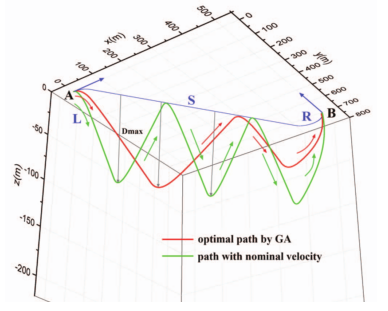
\includegraphics[width=.45\linewidth]{Shortest3DPath}} \quad
%     \subfloat[Shortest3DPath]
%     {\label{fig:Shortest3DPath2}
%     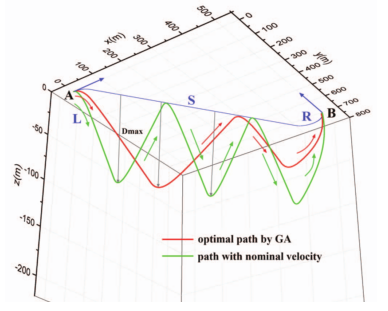
\includegraphics[width=.45\linewidth]{Shortest3DPath}}
% \caption{\hl{Shortest3DPath}.}
% \label{fig:Shortest3DPath}
% \end{figure}

\begin{equation}
\label{eq:CombinedLengthMetric}
	\rho\left( q_i, q_j \right) = \rho_h\left( q_i, q_j \right) + \rho_v\left( q_i,
	q_j \right)
	\text{,}
\end{equation}

\noindent where the first term corresponds to sum of the $n$ Dubins sectors
lengths, which are required to connect $q_i$ and $q_j$ in the horizontal plane,
and the second term corresponds to the distance in the heave (vertical) motion:

\begin{equation}
%\label{eq:CombinedLengthMetric}
	\rho_v\left( q_i, q_j \right) = \left | q_{iz} - q_{jz} \right|
\end{equation}

All this together, \ie the mathematical formulation, the use of the Dubins
curves over a $4D$ space, and the corresponding metrics for calculating
distances between different configurations, establish an alternative approach to
calculate \ac{3D} motions for torpedo-shaped \acp{AUV} under motion constraints.
Note that in the \ac{3D} case, we no longer have an analytical solution for the
shortest path between two poses. However, under the assumption that the \ac{AUV}
moves with a constant surge speed, the \ac{RRT*} algorithm will, with the
distance metric defined above, converge on the shortest path that satisfies the
descent speed constraint. The next section presents different simulation tests
that seeks to prove the validity of this approach.

\section{Results}

This section presents and discusses simulations of the Sparus~II \ac{AUV}
conducting \ac{3D} start-to-goal missions in different scenarios. Similarly as
it was done in the previous chapter, the solution paths have been calculated
under both geometric and differential constraints, in order to better understand
the importance of considering the \ac{AUV} motion capabilities when navigating
in complex environments. In all cases, the environment was assumed to be
pre-explored, \ie a map of the surroundings was available.

\subsection{Conducting 3D Missions under Geometric Constraints}

As it was explained before, Sparus~II is a torpedo-shaped \ac{AUV} equipped with
an independent vertical thruster that allows decoupling the horizontal and
vertical motions. This means that the vehicle is capable of descending or
ascending without needing to move forward or backward. For example, if a
start-to-goal query is defined as $q_{start} = [x_0, y_0, z_0, \psi_0]$ and
$q_{goal} = [x_0, y_0, z_0+depth, \psi_0]$, and the planner only takes into
account geometric constraints, the solution path should be one that connects
both configurations with a straight descent trajectory (see
Fig.~\ref{fig:S2StraightDescentWithoutPitch}).

\begin{figure}[htbp]
	\centering
	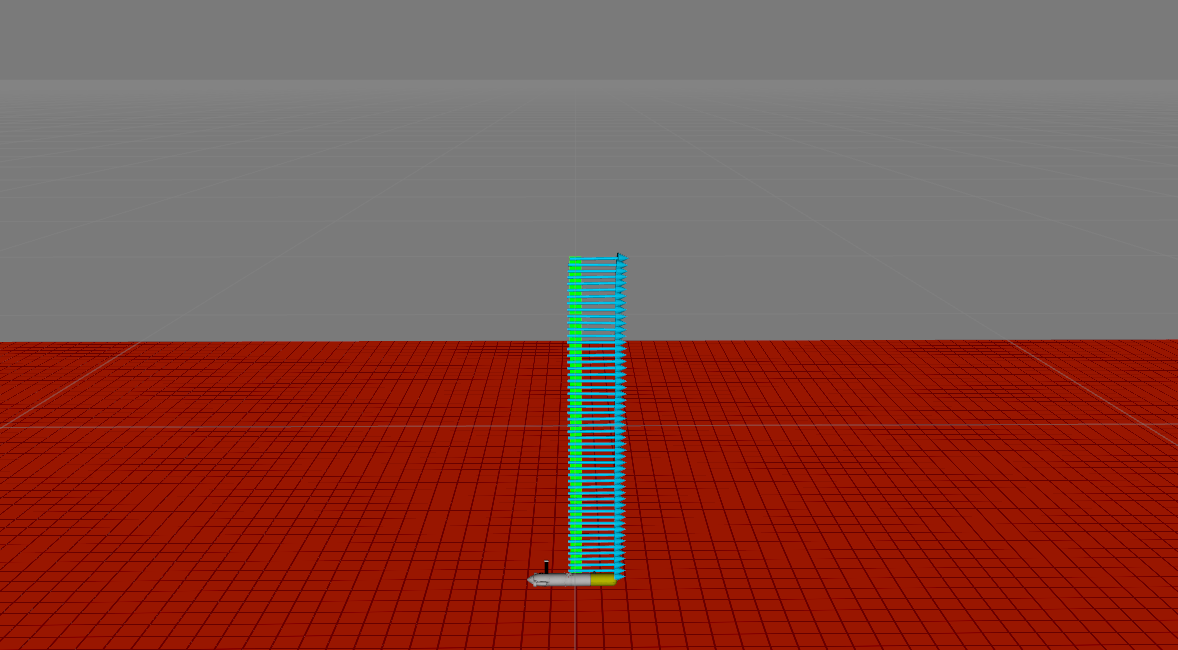
\includegraphics[width=.53\linewidth]{S2StraightDescentWithoutPitch}
\caption[3D Start-to-goal query that requires a straight descent trajectory.]
{Start-to-goal query that is defined as  $q_{start} = [x_0, y_0, z_0,
\psi_0]$ and $q_{goal} = [x_0, y_0, z_0+depth, \psi_0]$. The solution path (in
green) is calculated only taking into account geometric constraints, and
requires the AUV to follow a straight descent trajectory (in light blue).}
\label{fig:S2StraightDescentWithoutPitch}
\end{figure}

Let us define now a start-to-goal query where $q_{start} = [x_0, y_0,
z_0, \psi_0]$ and $q_{goal} = [x_0+distance, y_0, z_0+depth, \psi_0]$, which
means that the vehicle must conduct forward and vertical motions simultaneously.
Furthermore, let us assume that the vehicle is required to navigate at a constant
surge speed ($v$), as occurs in several \ac{AUV} applications. Under such
constraints, the time required to travel the horizontal distance can be
calculated as $t_h = \frac{distance}{v}$, while the descending speed ($d$) can
be adjusted up to a maximum value ($d_{max}$), which can be calculated as $d =
\frac{depth}{t_h}$. This kind of tasks could also be tackled with geometric
constraints, however there may be situations in which the resulting path cannot
be followed by the \ac{AUV}. For example, if $t_h$ allows enough time to descend
the desired vertical distance, \ie $d <= d_{max}$, the vehicle will successfully
complete the task, otherwise it may not reach the desired depth (see
Fig.~\ref{fig:S2DescentConstraint}).

\begin{figure}[htbp]
    \myfloatalign
    \subfloat[Successful query]
    {\label{fig:S2DescentConstraintValid}
    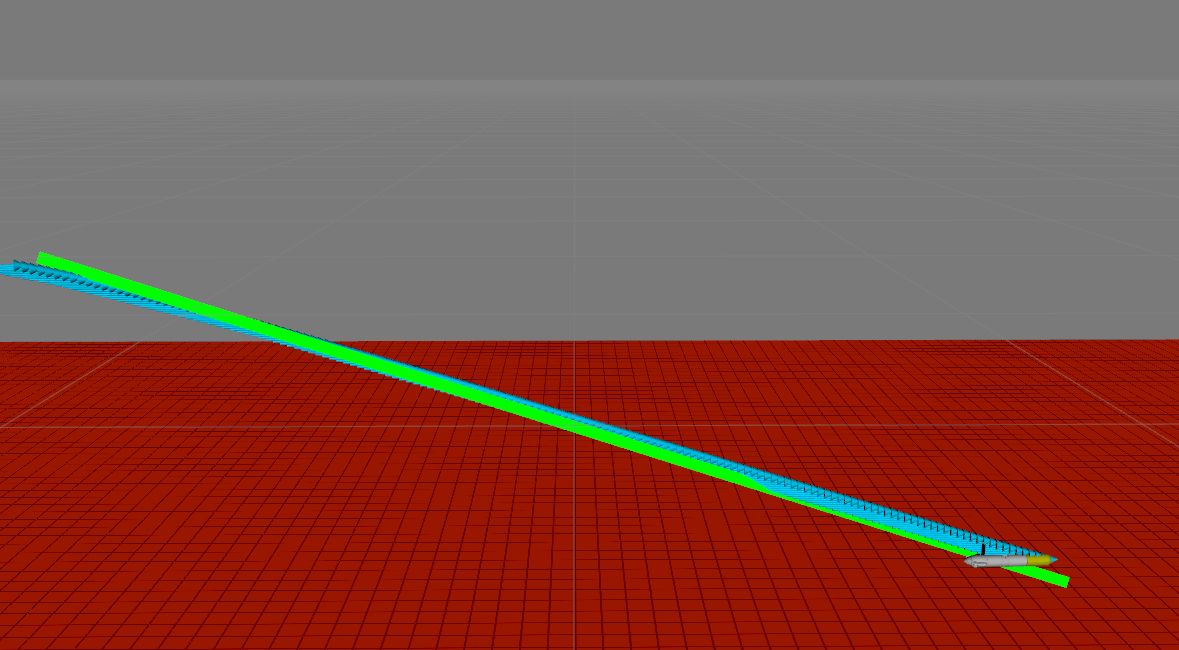
\includegraphics[width=.45\linewidth]{S2DescentConstraintValid}} \quad
    \subfloat[Unsuccessful query]
    {\label{fig:S2DescentConstraintNoValid}%
     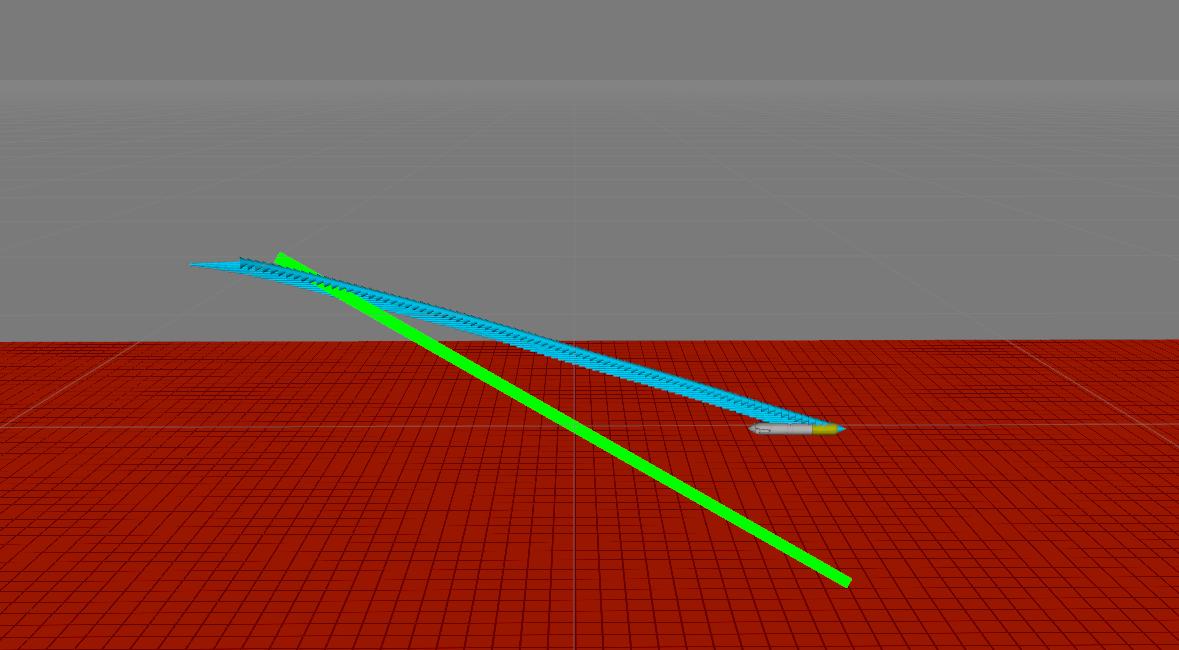
\includegraphics[width=.45\linewidth]{S2DescentConstraintNoValid}}
\caption[3D Start-to-goal query that requires forward and vertical motion.]
{Start-to-goal queries that are defined as $q_{start} = [x_0, y_0,
z_0, \psi_0]$ and $q_{goal} = [x_0+distance, y_0, z_0+depth, \psi_0]$. The
solution path (in green) is calculated only taking into account geometric
constraints, and requires the AUV to conduct forward and vertical motion
(in light blue). The Sparus~II is assumed to have a constant surge speed
$v=0.6m/s$, and a maximum descending speed $d_{max}=0.2m/s$.
\protect \subref{fig:S2DescentConstraintValid} Successful query with
$distance=20m$ and $depth=6m$.
\protect \subref{fig:S2DescentConstraintNoValid} Unsuccessful query
with $distance=10m$ and $depth=6m$.}
\label{fig:S2DescentConstraint}
\end{figure}

Previous examples did not require the \ac{AUV} to change its position along the
sway direction, and therefore a constant orientation was assumed during the
mission. Nonetheless, real missions, especially those intended for this thesis,
present more challenging scenarios. In such cases, the vehicle probably needs
not only to vary its vertical position, but also to change its orientation in
order to conduct turning maneuvers.

Figure~\ref{fig:S2PlannOffBlocksRRTstarGeom3D} depicts a test scenario that is
composed of two blocks ($12m \times 12m \times 8m$), which are separated by a
passage of $4m$. Over this simulated environment, a start-to-goal query solution and its
execution are presented, where $q_{start} = [x_0, y_0, z_0]$ and $q_{goal} =
[x_1, y_1, z_1]$, which means that the orientation was not taken into account.
The \ac{3D} solution path was calculated using an \ac{RRT*} algorithm under
geometric constraints, and it was followed by the simulated Sparus~II. It can be
observed that, although the change of depth did not require a descending speed
greater than the vehicle capabilities (\ie $d<d_{max}$), the vehicle followed a
trajectory that was not initially planned, especially when conducting turning
maneuvers. This was mainly due to the fact that the planner did not consider the
vehicle's motion constraints. Next sections will demonstrate how the use of the
extended \ac{3D} Dubins curves approach, explained before, can overcome these
situations.

\begin{figure}[htbp]
    \myfloatalign
    \subfloat[Query top view]
    {\label{fig:S2PlannOffBlocksRRTstarGeom3D_top}
    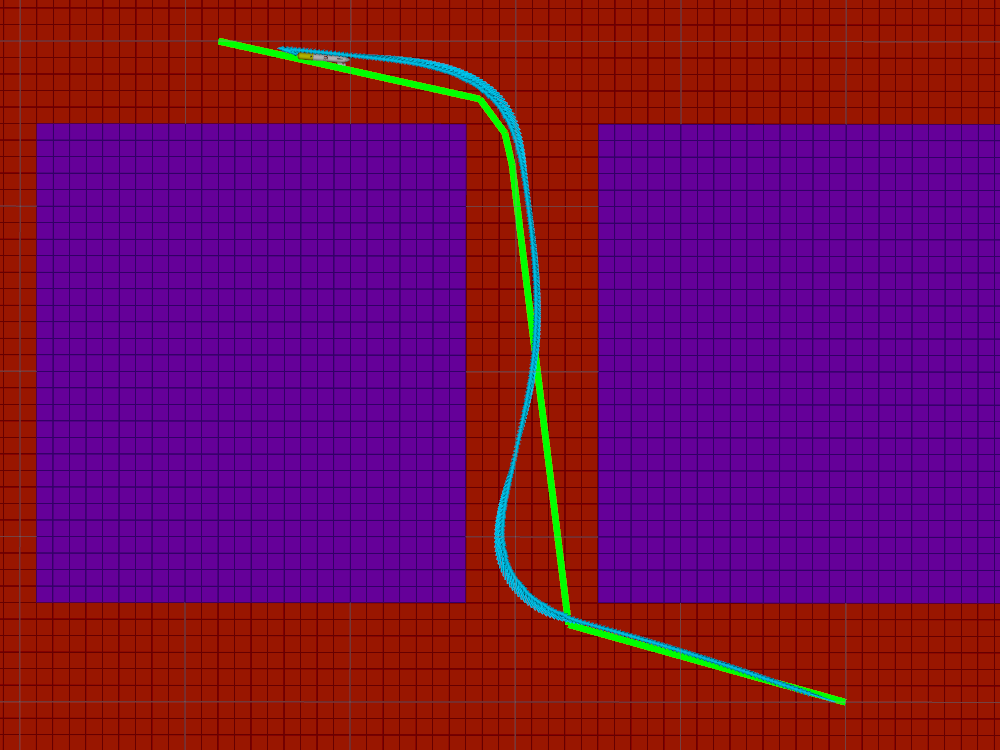
\includegraphics[width=.65\linewidth]{S2PlannOffBlocksRRTstarGeom3D_top}} \quad
    \subfloat[Query front view]
    {\label{fig:S2PlannOffBlocksRRTstarGeom3D_front}
    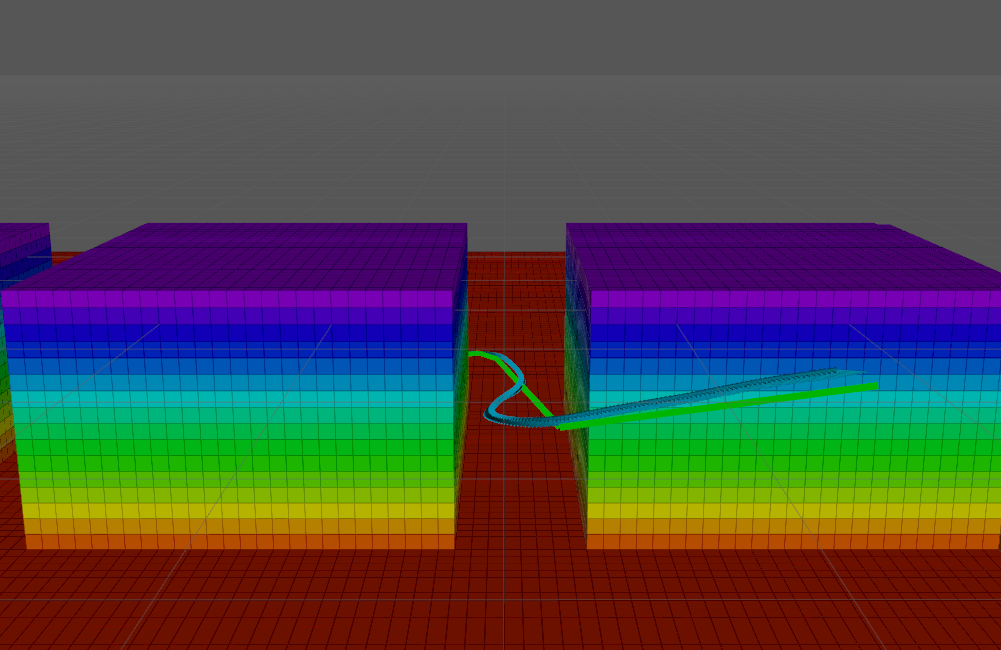
\includegraphics[width=.65\linewidth]{S2PlannOffBlocksRRTstarGeom3D_front}} \quad
    \subfloat[Query back view]
    {\label{fig:S2PlannOffBlocksRRTstarGeom3D_back}%
     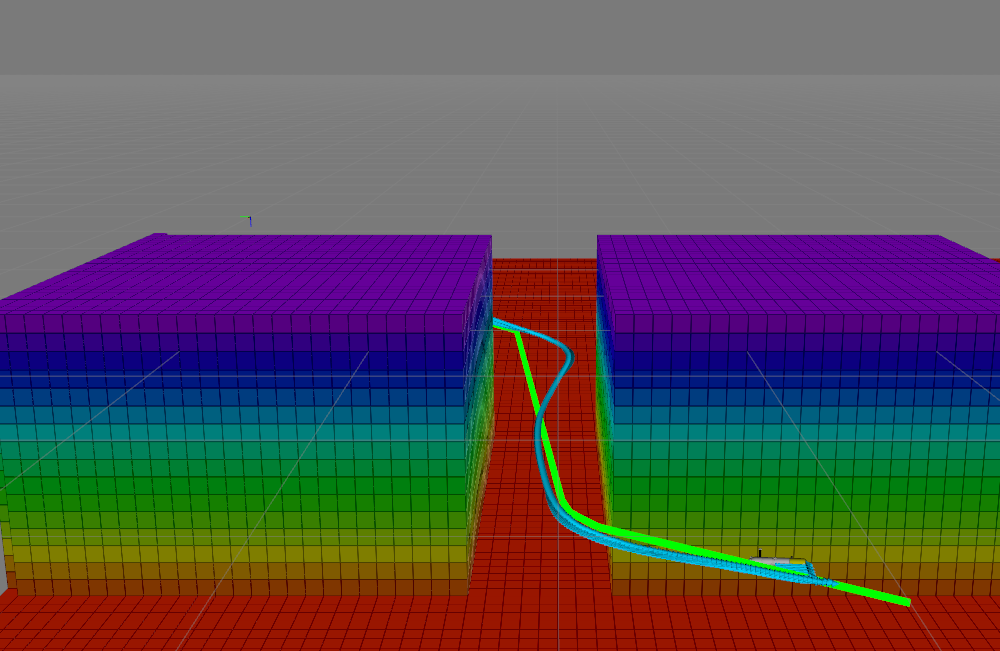
\includegraphics[width=.65\linewidth]{S2PlannOffBlocksRRTstarGeom3D_back}}
\caption[Simulation of the Sparus~II AUV attempting to follow a 3D solution path
calculated by an RRT* under geometric constraints.]
{Simulated environment composed of two blocks ($12m \times 12m \times 8m$),
where a start-to-goal query is defined as $q_{start} = [x_0, y_0, z_0]$ and $q_{goal} =
[x_1, y_1, z_1]$. The solution path (in green) is calculated only taking into
account geometric constraints. A simulated Sparus~II AUV attempted to follow the
path, however the resulting trajectory (in light blue) differs from the one
calculated, thus leading to risky situations when conducting turning maneuvers.}
\label{fig:S2PlannOffBlocksRRTstarGeom3D}
\end{figure}


\subsection{Conducting 3D Missions under Motion Constraints}

The previous section presented as a first example, a simulated task in which the
Sparus~II \ac{AUV} was required to conduct a vertical motion while attempting to
maintain its orientation invariant (see
Fig.~\ref{fig:S2StraightDescentWithoutPitch}). Let us now assume that the vehicle
has to solve the same task, \ie a start-to-goal query defined as $q_{start} =
[x_0, y_0, z_0, \psi_0]$ and $q_{goal} = [x_0, y_0, z_0+depth, \psi_0]$; but
this time the vehicle has to navigate with a constant surge speed $v$ and a
descending speed up to a maximum value $d_{max}$. Under such constraints, the
motion planner must find a solution that combines turning and descending
maneuvers to reach the final position and orientation. This problem can be
solved with the extended Dubins curves approach that has been explained
throughout previous sections. One possible solution, where the vehicle
circumnavigates while descending to reach the desired depth and orientation, can
be observed in Fig.~\ref{fig:CircDescDubinsRRTstar3D}. Furthermore, this
solution is near-optimal under the assumption of a constant surge speed.


\begin{figure}[htbp]
    \myfloatalign
    \subfloat[Query top view]
    {\label{fig:CircDescDubinsRRTstar3D_Top}
    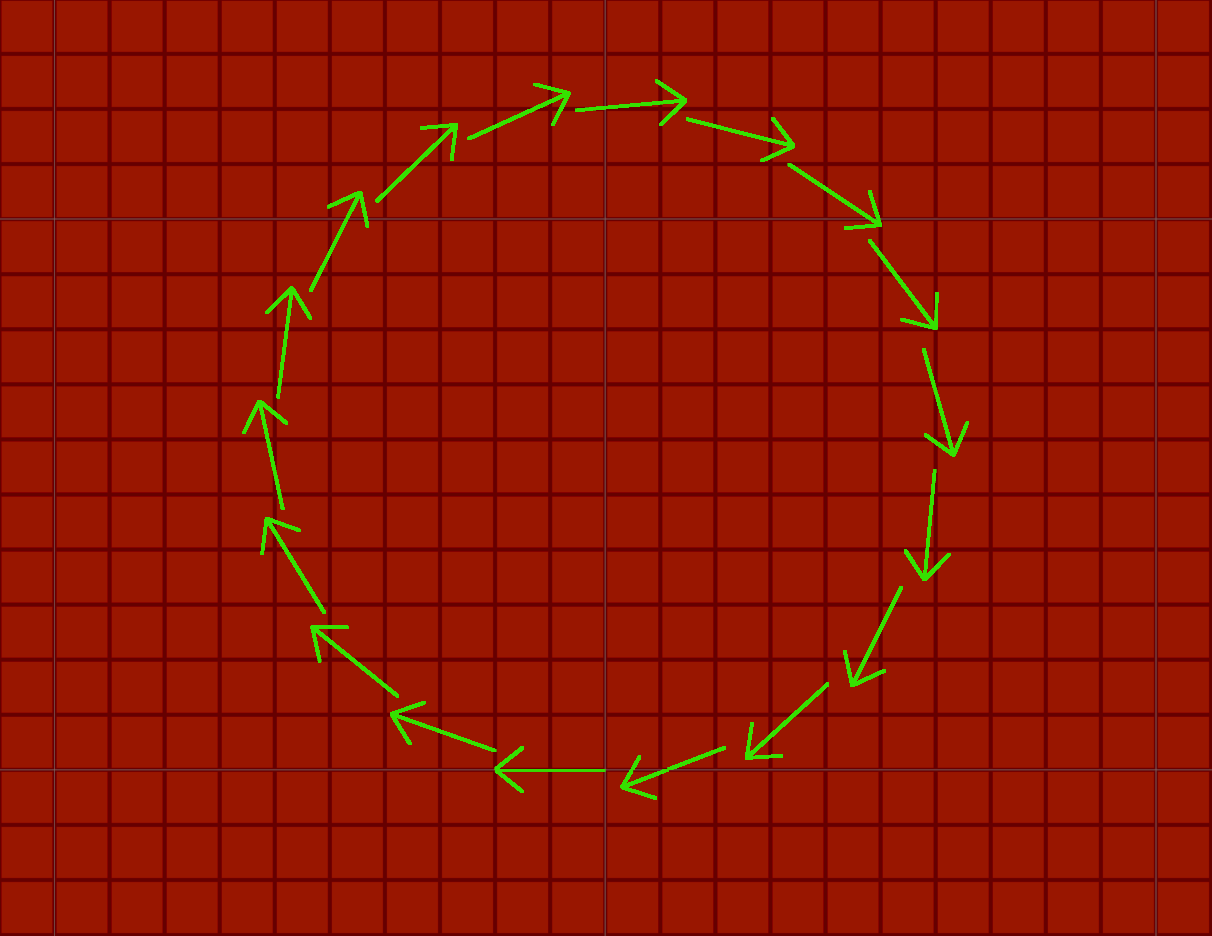
\includegraphics[width=.45\linewidth]{CircDescDubinsRRTstar3D_Top}} \quad
    \subfloat[Simulation top view]
    {\label{fig:CircDescDubinsRRTstar3D_Top_}%
     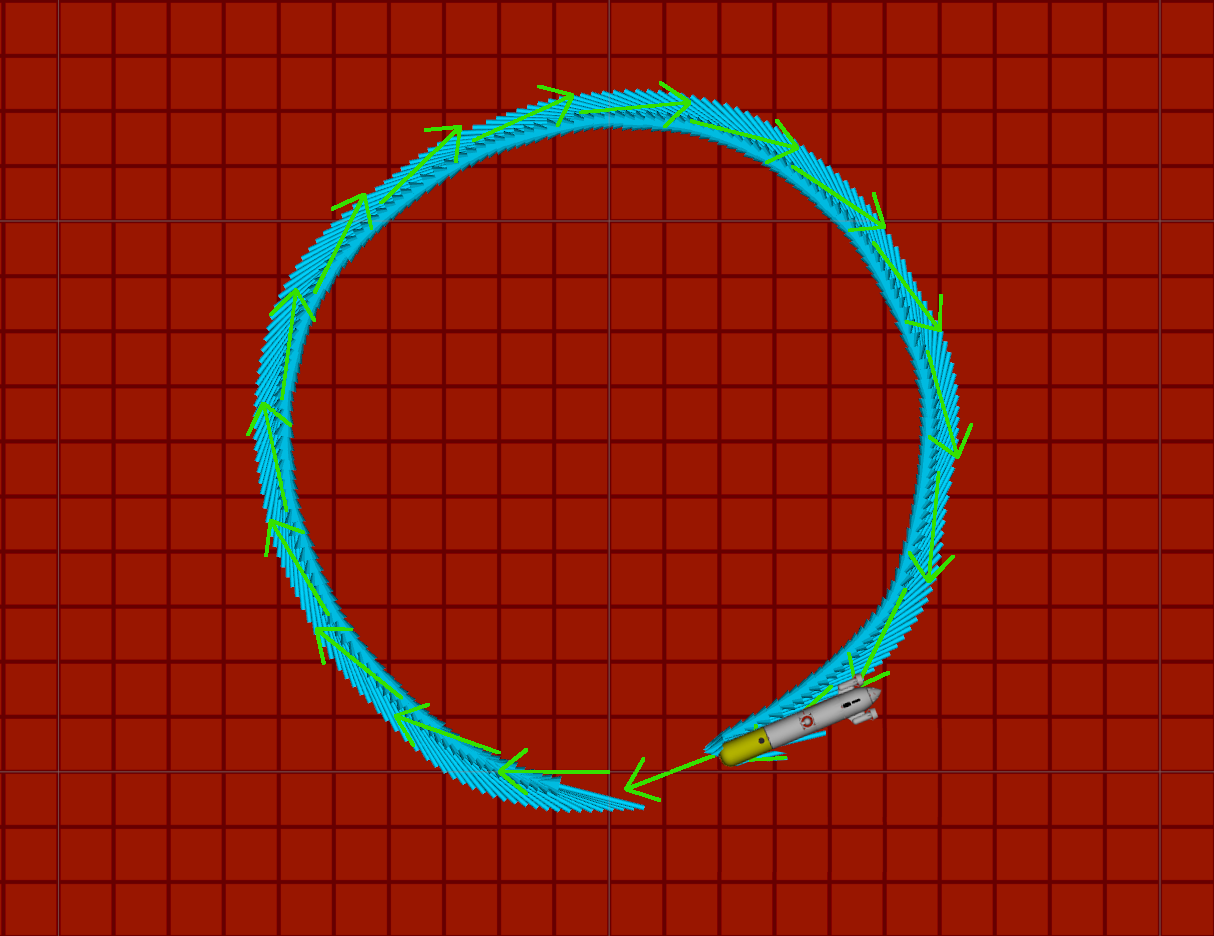
\includegraphics[width=.45\linewidth]{CircDescDubinsRRTstar3D_Top_}}\\
%      \subfloat[CircDescDubinsRRTstar3D 41]
%     {\label{fig:CircDescDubinsRRTstar3D_41}
%     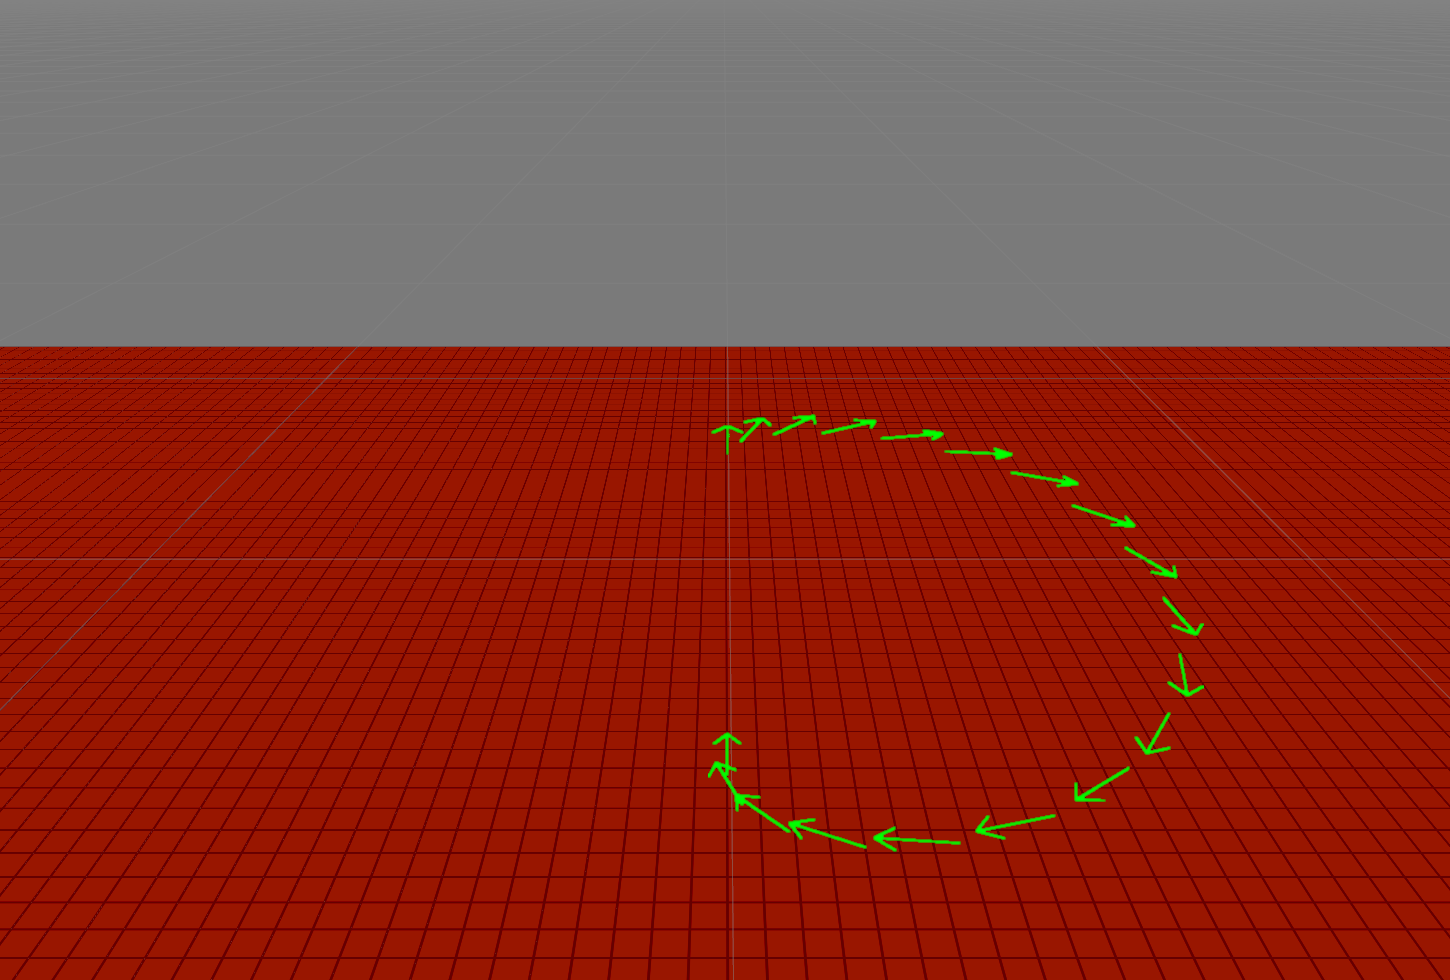
\includegraphics[width=.45\linewidth]{CircDescDubinsRRTstar3D_41}} \quad
%     \subfloat[CircDescDubinsRRTstar3D 41]
%     {\label{fig:CircDescDubinsRRTstar3D_41_}%
%      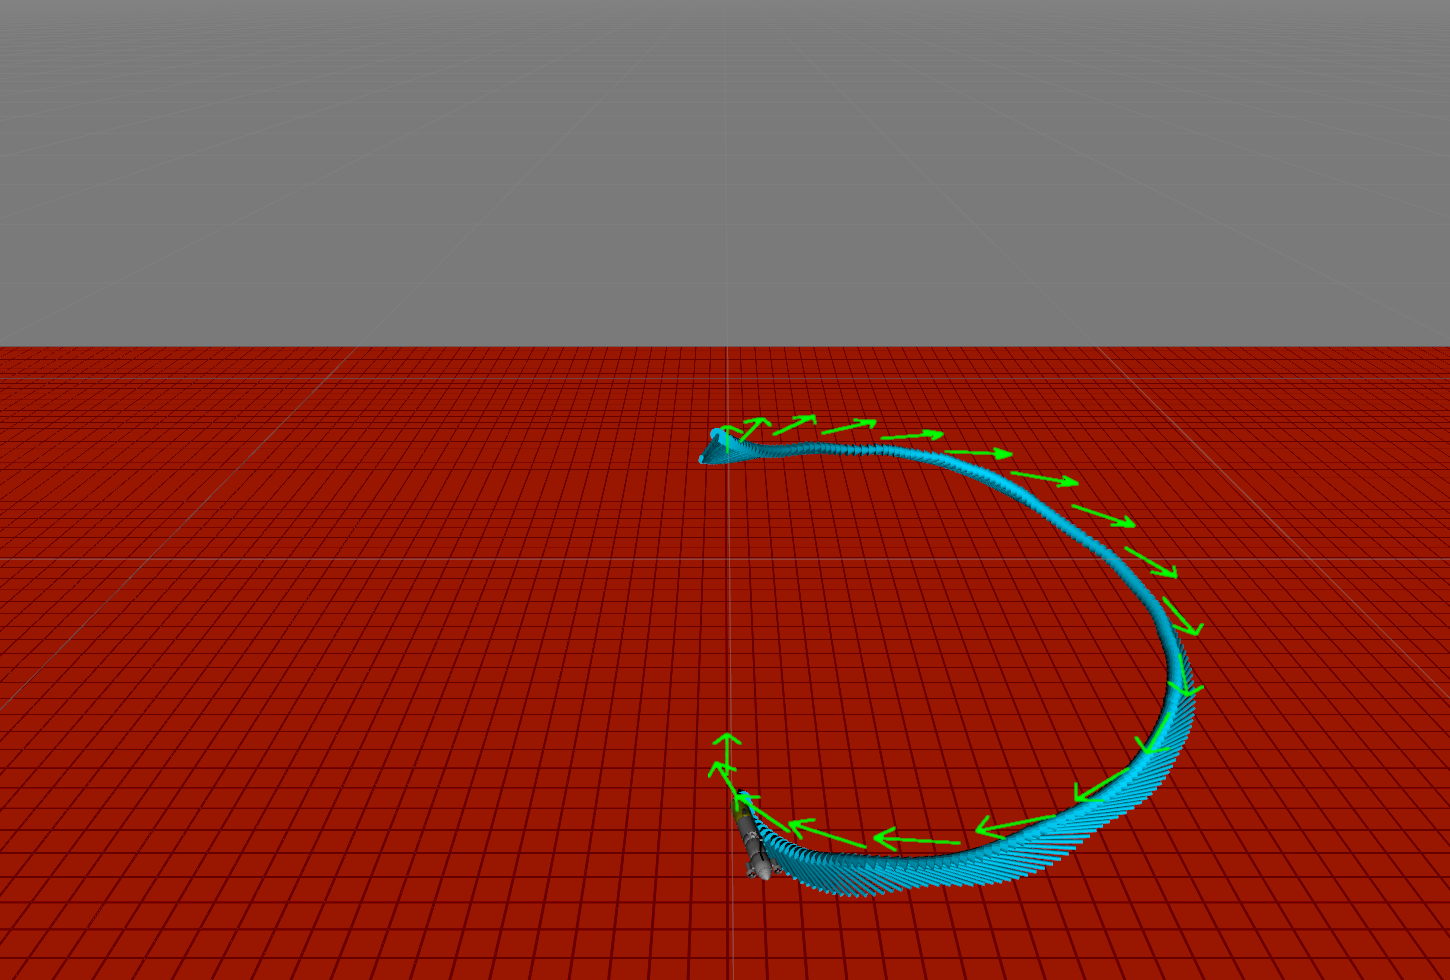
\includegraphics[width=.45\linewidth]{CircDescDubinsRRTstar3D_41_}}\\
     \subfloat[Query perspective view]
    {\label{fig:CircDescDubinsRRTstar3D_11}
    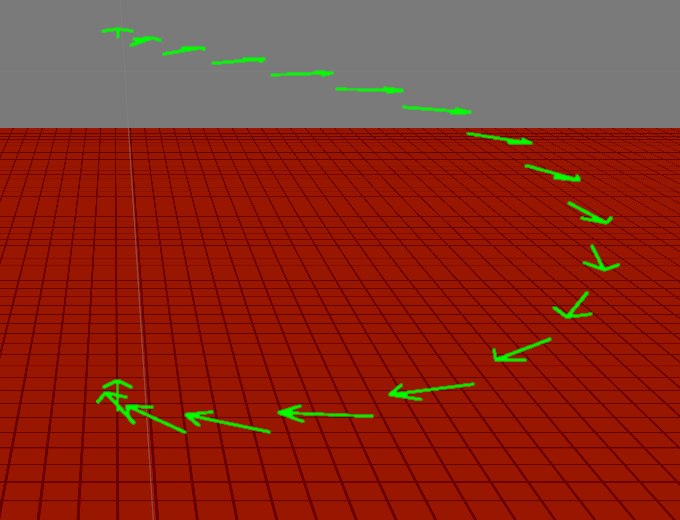
\includegraphics[width=.45\linewidth]{CircDescDubinsRRTstar3D_11}} \quad
    \subfloat[Simulation perspective view]
    {\label{fig:CircDescDubinsRRTstar3D_11_}%
     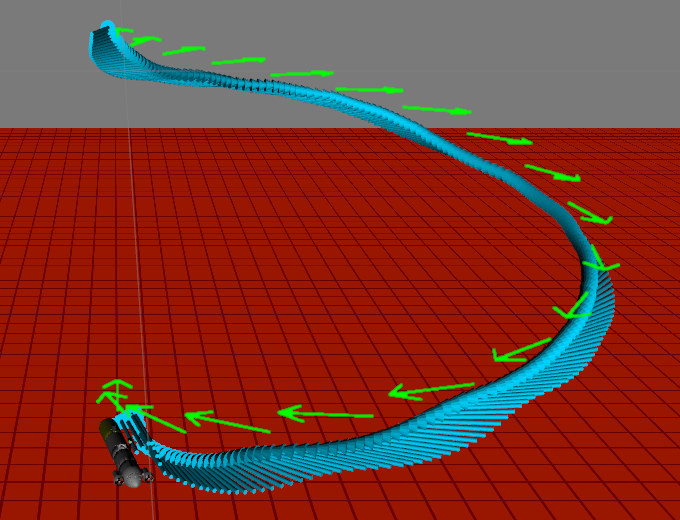
\includegraphics[width=.45\linewidth]{CircDescDubinsRRTstar3D_11_}}
\caption[3D Start-to-goal query that requires circumnavigating while descending
to reach the desired depth and orientation.]
{Start-to-goal query that is defined as $q_{start} = [x_0, y_0, z_0, \psi_0]$
and $q_{goal} = [x_0, y_0, z_0+depth, \psi_0]$. The AUV is assumed to navigate
at a constant surge speed $v$, and a descending speed up to $d_{max}$. The
solution path (in green) is calculated with an RRT* that uses the extended
Dubins curves, which incorporate the vehicle 3D motion capabilities. The
simulated Sparus~II successfully describes a helical trajectory (in light blue)
that follows the calculated path.}
\label{fig:CircDescDubinsRRTstar3D}
\end{figure}

Figure~\ref{fig:S2PlannOffBlocksRRTstarDubins3D} presents the same test scenario
composed of two blocks separated by a narrow passage used in the previous
section. Similarly as occurred in the simulation presented in
Fig.~\ref{fig:S2PlannOffBlocksRRTstarGeom3D}, the start-to-goal query requires
the vehicle to completely change its \ac{3D} position, but this time it also
specifies the desired \ac{AUV} heading. This task, for which the vehicle is also
under the surge and descending speeds constraints mentioned before, consists
of a $q_{start} = [x_0, y_0, z_0, \psi_0]$ and a $q_{goal} = [x_1, y_1, z_1,
\psi_1]$. This time the resulting vehicle trajectory coincides with the planned
path, even when conducting turning maneuvers.

\begin{figure}[htbp]
    \myfloatalign
    \subfloat[Query top view]
    {\label{fig:S2PlannOffBlocksRRTstarDubins3D_top}
    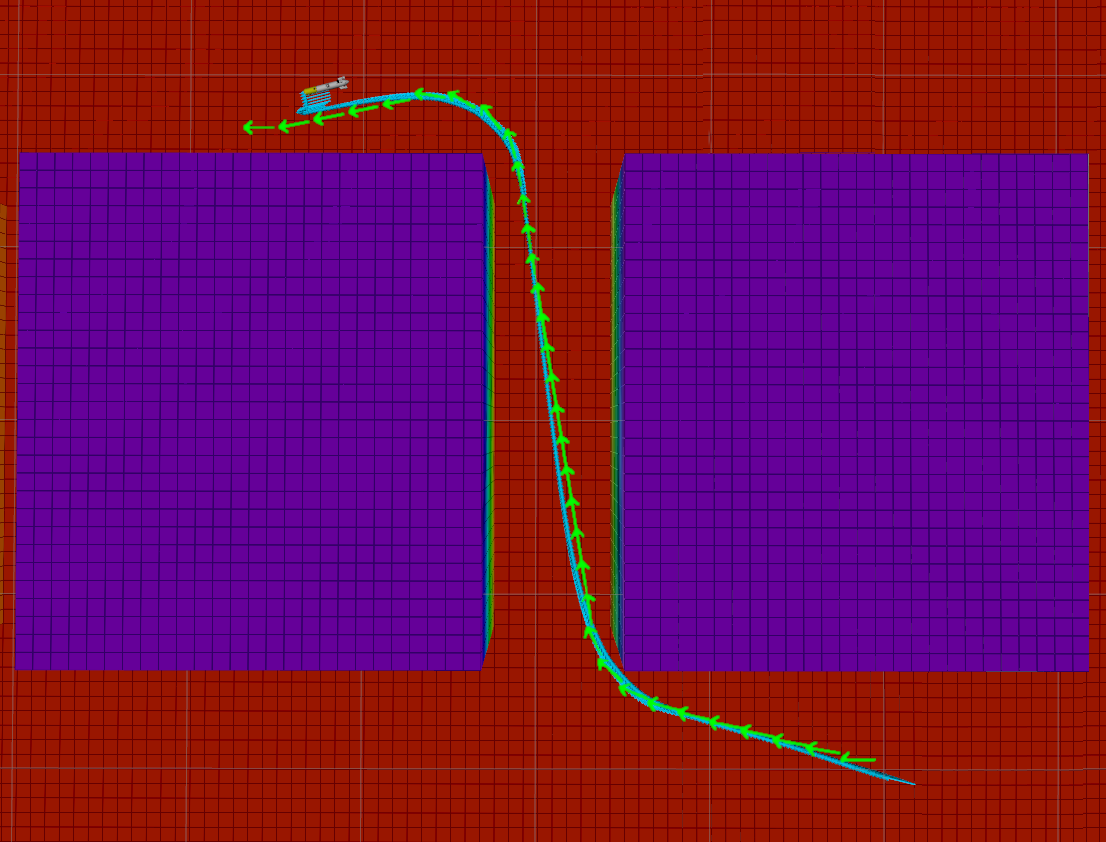
\includegraphics[width=.65\linewidth]{S2PlannOffBlocksRRTstarDubins3D_top}} \quad
    \subfloat[Query front view]
    {\label{fig:S2PlannOffBlocksRRTstarDubins3D_front}
    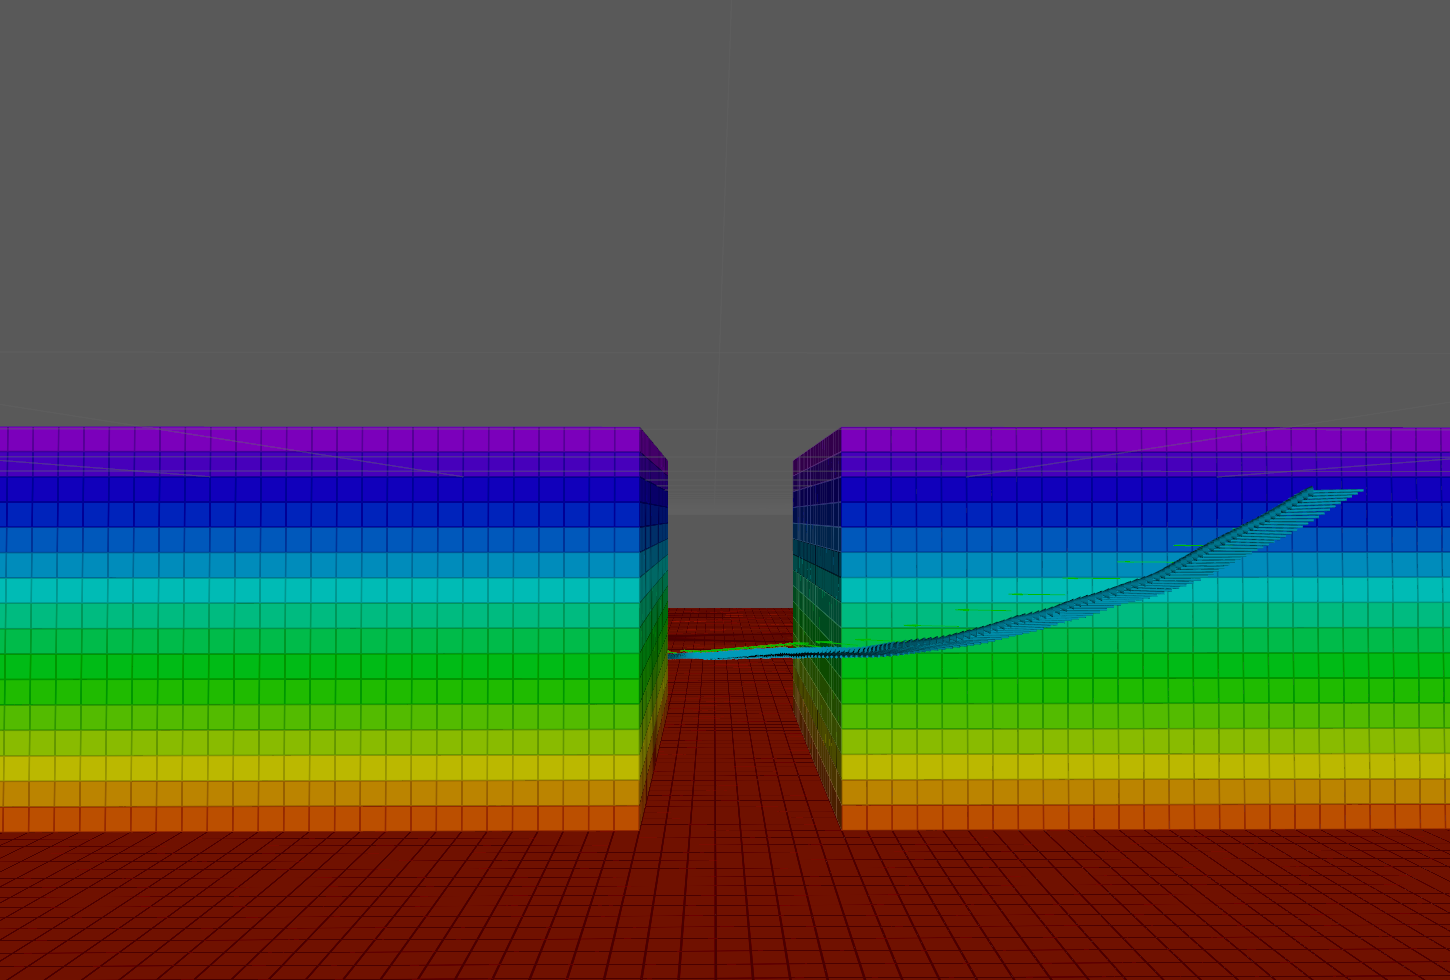
\includegraphics[width=.65\linewidth]{S2PlannOffBlocksRRTstarDubins3D_front}} \quad
    \subfloat[Query back view]
    {\label{fig:S2PlannOffBlocksRRTstarDubins3D_back}%
     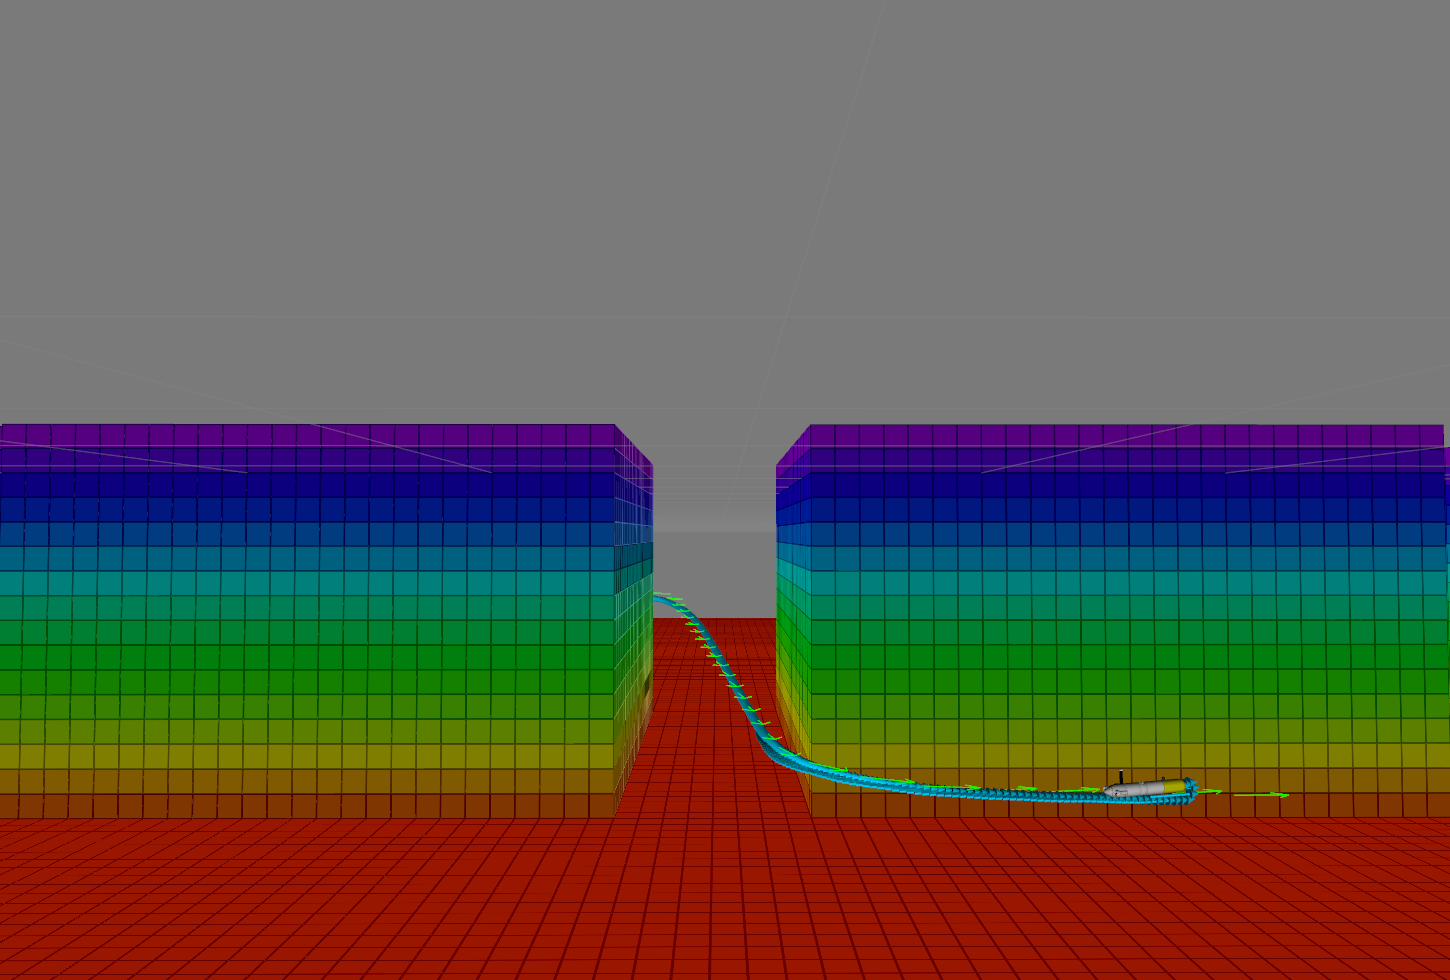
\includegraphics[width=.65\linewidth]{S2PlannOffBlocksRRTstarDubins3D_back}}
\caption[Simulation of the Sparus~II AUV attempting to follow a 3D solution path
calculated by an RRT* that uses the extended Dubins curves approach.]
{Simulated environment composed of two blocks ($12m \times 12m \times 8m$),
where a start-to-goal query is defined as $q_{start} = [x_0, y_0, z_0, \psi_0]$ and
$q_{goal} = [x_1, y_1, z_1, \psi_1]$. The solution path (in green) is calculated
by an RRT* that uses the extended Dubins curves approach. A simulated Sparus~II
AUV describes a trajectory (in light blue), which does not differ significantly
from the one calculated, even when conducting turning maneuvers.}
\label{fig:S2PlannOffBlocksRRTstarDubins3D}
\end{figure}

Finally, in order to completely assess the extended Dubins approach for \ac{3D}
motions, Figure~\ref{fig:S2PlannOffSeamountRRTstDubins3D} depicts a
start-to-goal mission in a high-relief environment. The requested query has been
defined in such a way, that any solution path would require the \ac{AUV} to
conduct turning, ascending and descending maneuvers. The resulting path and its
corresponding execution by the simulated Sparus~II \ac{AUV} was successful, thus
completely proving the presented approach capabilities.

There are, however, some aspects that have to be addressed in order to make this
approach really useful for the proposed applications. The first of them is that
the intended usage scenarios involve generally unexplored spaces, which means
that a map is not available. A second aspect is the safety of the vehicle, which
can be compromised when navigating in close proximity to the obstacles. These
and other aspects, as well as the different strategies proposed to cope with
them, will be discussed in detail in the next chapter.

\begin{figure}[htbp]
    \myfloatalign
    \subfloat[]
    {\label{fig:S2PlannOffSeamountRRTstDubins3D_Top}
    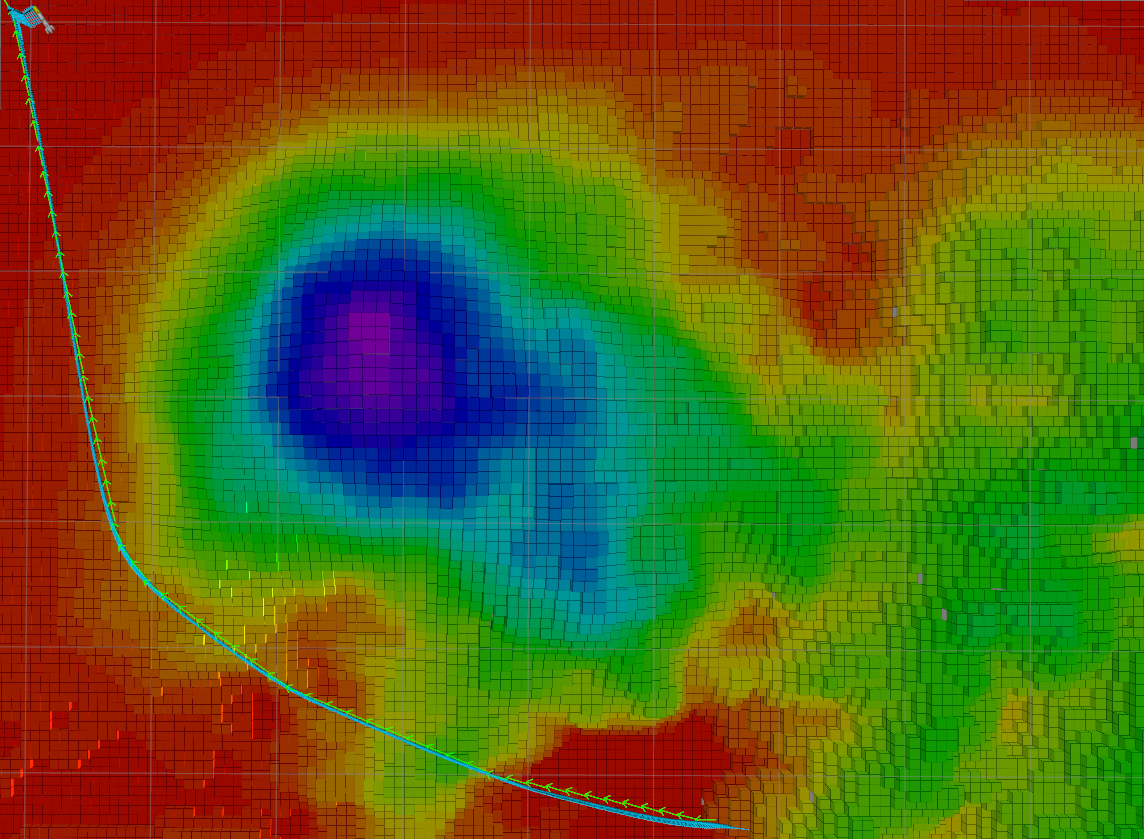
\includegraphics[width=.45\linewidth]{S2PlannOffSeamountRRTstDubins3D_Top}} \quad %\\
%      \subfloat[]
%     {\label{fig:S2PlannOffSeamountRRTstDubins3D_A}
%     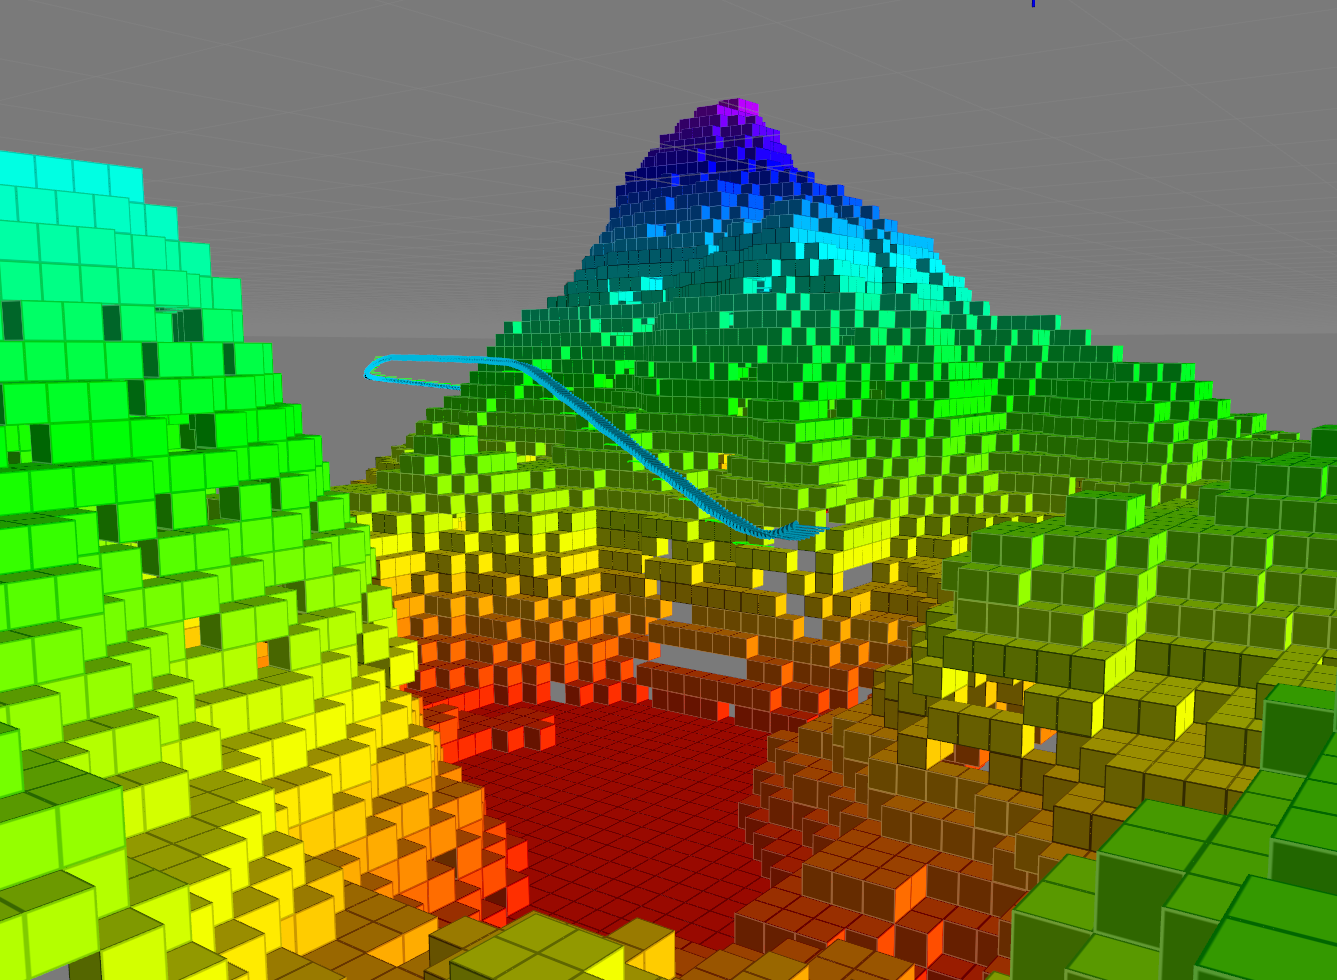
\includegraphics[width=.45\linewidth]{S2PlannOffSeamountRRTstDubins3D_A}} \quad
    \subfloat[]
    {\label{fig:S2PlannOffSeamountRRTstDubins3D_B}%
     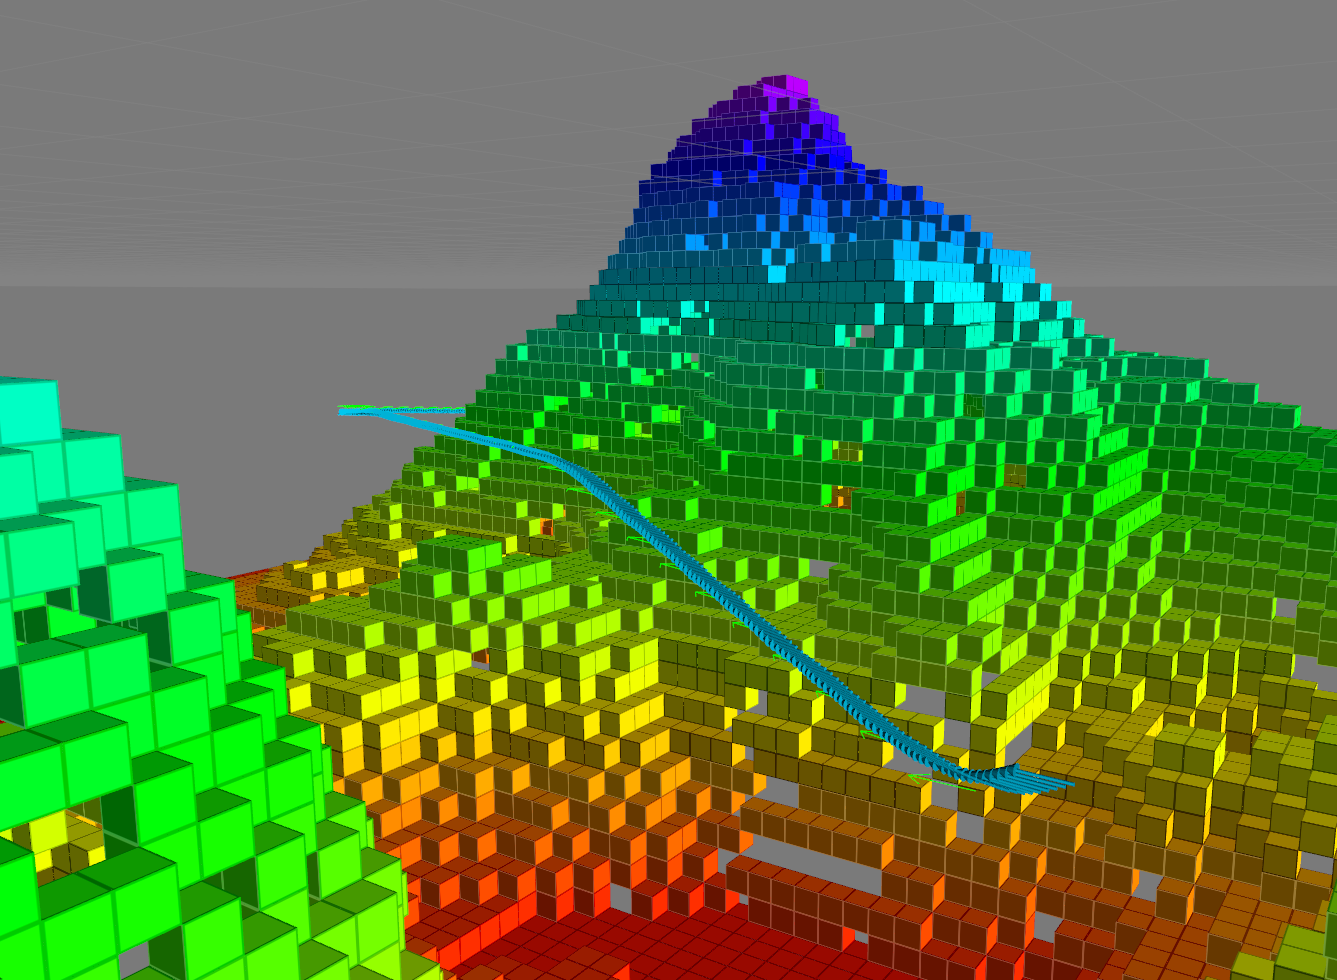
\includegraphics[width=.45\linewidth]{S2PlannOffSeamountRRTstDubins3D_B}}\\
     \subfloat[]
    {\label{fig:S2PlannOffSeamountRRTstDubins3D_C}
    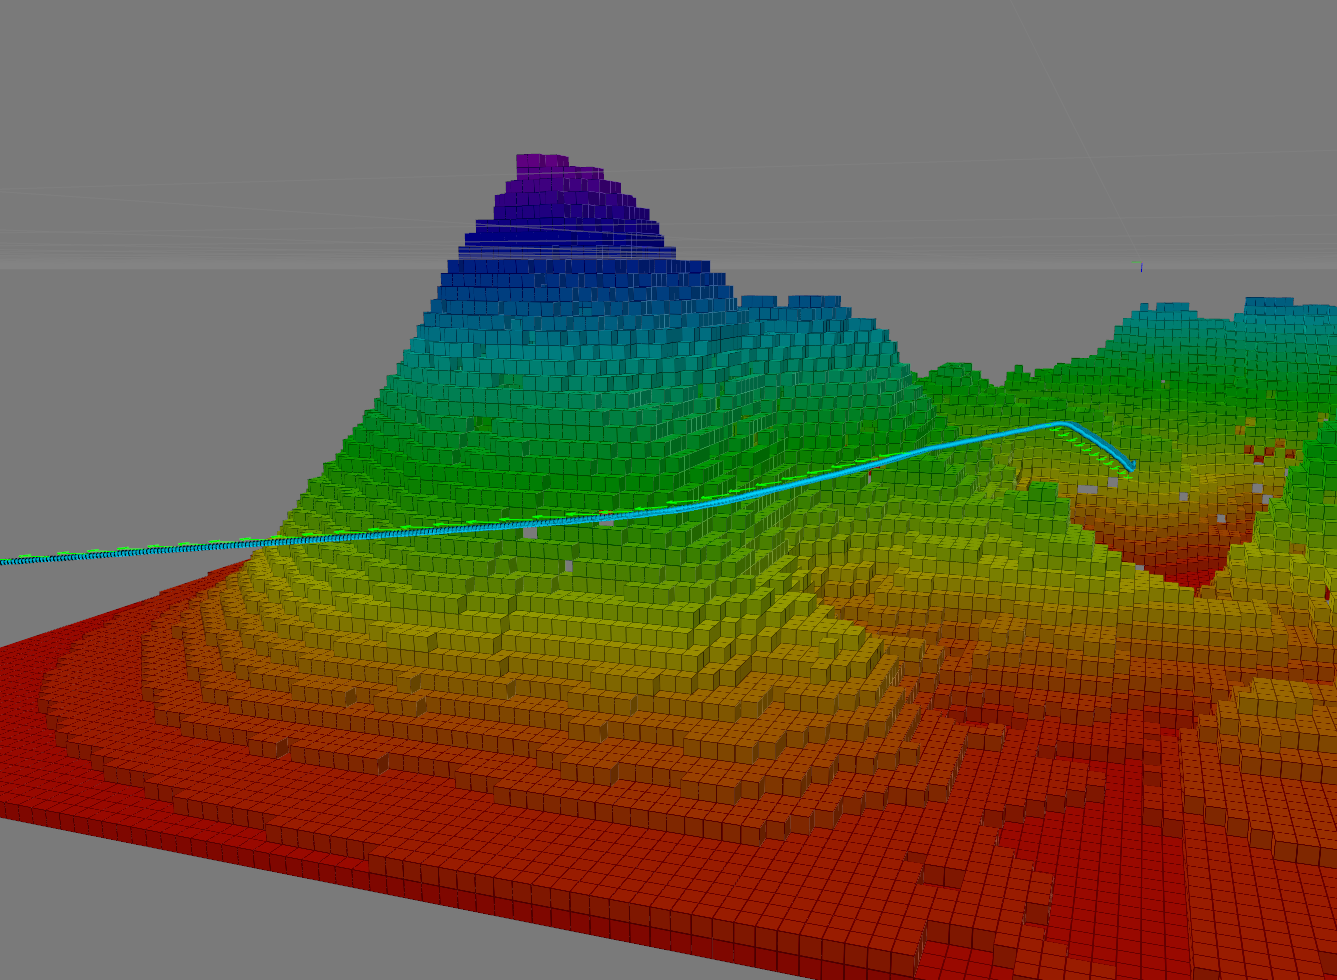
\includegraphics[width=.45\linewidth]{S2PlannOffSeamountRRTstDubins3D_C}} \quad
    \subfloat[]
    {\label{fig:S2PlannOffSeamountRRTstDubins3D_D}%
     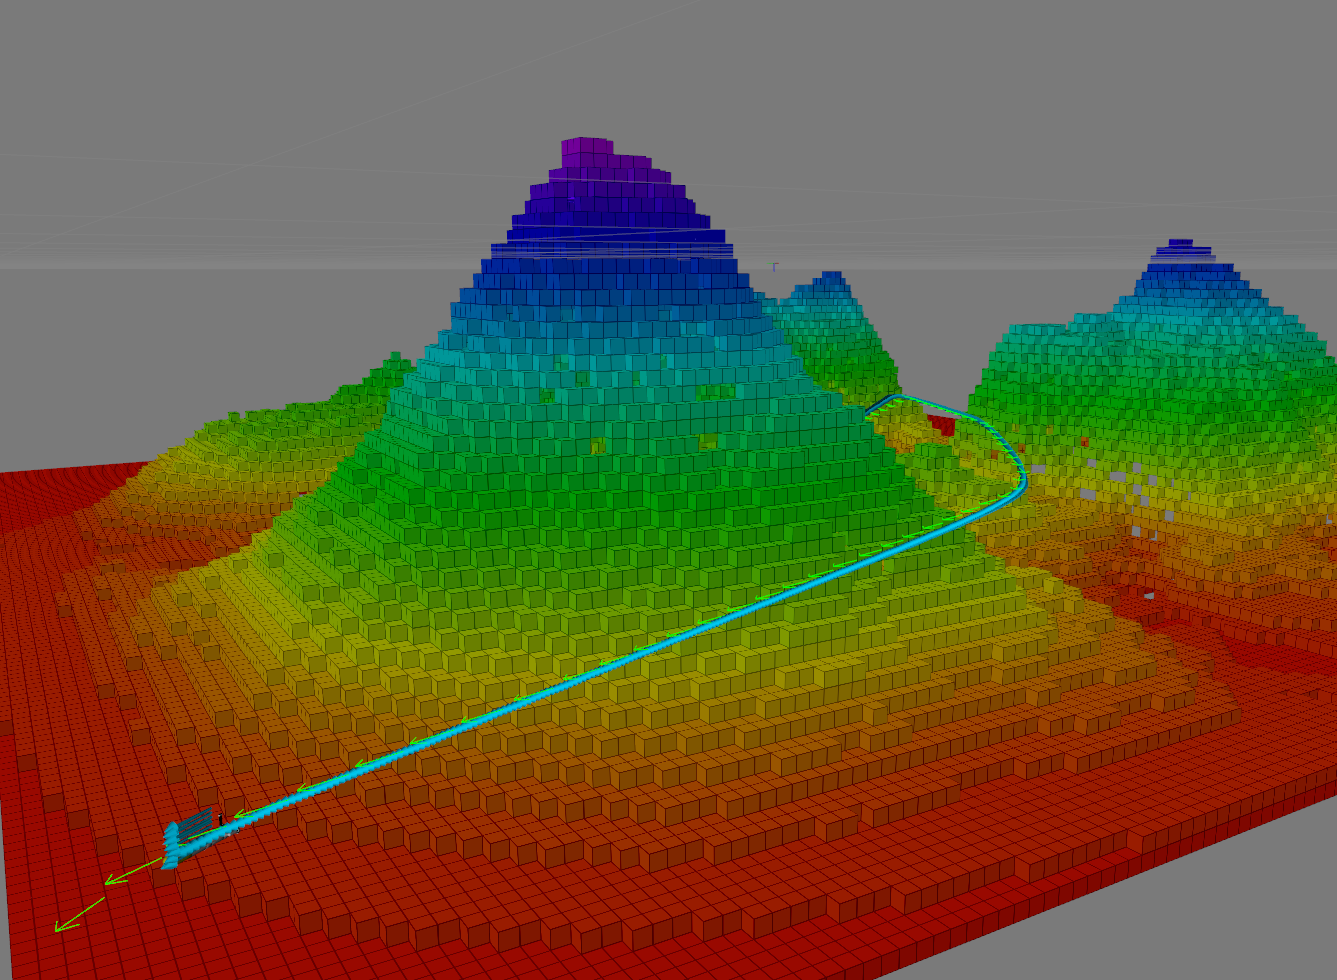
\includegraphics[width=.45\linewidth]{S2PlannOffSeamountRRTstDubins3D_D}}
\caption[Simulation of the Sparus~II AUV attempting to follow a 3D solution path
in a high-relief environment. The path is calculated by an RRT* that uses the
extended Dubins curves approach.]
{High-relief simulated environment composed of multiple seamounts, where a
start-to-goal query is defined as $q_{start} = [x_0, y_0, z_0, \psi_0]$ and
$q_{goal} = [x_1, y_1, z_1, \psi_1]$. A simulated Sparus~II AUV describes a
trajectory (in light blue), which attempts following a solution path that. This
path is calculated by an RRT*, which uses the extended Dubins curves approach.}
\label{fig:S2PlannOffSeamountRRTstDubins3D}
\end{figure}

% ---------------------------------------------------------------------------
%: ----------------------- end of thesis sub-document ------------------------
% ---------------------------------------------------------------------------

